%
% Copyright (C) 2004-2009 Jason Blevins <jrblevin@sdf.lonestar.org>
% http://jblevins.org/projects/cv-template/
%
% You may use use this document as a template to create your own CV
% and you may redistribute the source code freely. No attribution is
% required in any resulting documents. I do ask that you please leave
% this notice and the above URL in the source code if you choose to
% redistribute this file.

\documentclass[letterpaper, 11pt]{article}

\usepackage{hyperref}
\usepackage{geometry}

%%%%%%%%%%%%%%%%%%%%%%%%%%%%%%%%%%%%%%%%%%%%%%%%%%%%%%%%%%%%%%%%%%%%%%%%%%%%%%%%%
\usepackage[minbibnames=3,sorting=ndymdt,date=comp,isbn=false,doi=false,defernumbers=true,backend=biber]{biblatex}

% https://tex.stackexchange.com/a/408041
\NewBibliographyString{toappear}
\DefineBibliographyStrings{english}{%
  toappear = {to appear},
}

\renewbibmacro*{in:}{%
  \iffieldundef{pubstate}
    {}
    {\printfield{pubstate}%
     \setunit{\addspace}%
     \clearfield{pubstate}}%
  \printtext{%
    \bibstring{in}\intitlepunct}}

\addbibresource[]{papers.bib}
\addbibresource[]{presentations-conference.bib}
\addbibresource[]{presentations-invited.bib}
\addbibresource[]{presentations-other.bib}

\DeclareSortingTemplate{ndymdt}{
	\sort[direction=descending]{
		\field{sortyear}
		\field{year}
		\literal{9999}
	}
	\sort[direction=descending]{
		\field[padside=left,padwidth=2,padchar=0]{month}
		\literal{99}
	}
	\sort[direction=descending]{
		\field[padside=left,padwidth=2,padchar=0]{day}
		\literal{99}
	}
	\sort{
		\field{presort}
	}
	\sort[final]{
		\field{sortkey}
	}
	\sort{
		\field{sortname}
		\field{author}
		\field{editor}
		\field{translator}
		\field{sorttitle}
		\field{title}
	}
	\sort{
		\field{sorttitle}
	}
	\sort[direction=descending]{
		\field[padside=left,padwidth=4,padchar=0]{volume}
		\literal{9999}
	}
}

\usepackage{graphicx}



%\usepackage[sfdefault]{cabin}
%\usepackage[T1]{fontenc}

%\usepackage[sfdefault]{overlock} %% Option 'sfdefault' only if the base font of the document is to be sans serif
\usepackage[default,oldstyle,scale=0.95]{opensans}

\usepackage[T1]{fontenc}

\usepackage{enumitem}
\usepackage{setspace}
	\onehalfspacing
\usepackage{xcolor}

% Set your name here
\def\name{George G. Vega Yon, Ph.D.}

% Replace this with a link to your CV if you like, or set it empty
% (as in \def\footerlink{}) to remove the link in the footer:
\def\footerlink{https://ggvy.cl}

% The following metadata will show up in the PDF properties
\hypersetup{
  colorlinks = true,
  urlcolor = teal,
  pdfauthor = {\name},
  pdfkeywords = {statistics, mathematics, statistical computing, data science, machine learning},
  pdftitle = {\name: Curriculum Vitae},
  pdfsubject = {Curriculum Vitae},
  pdfpagemode = UseNone
}

\geometry{
%  body={6.5in, 9in},
  left=1in,
  top=1in,
  right=1in,
  bottom=1in
}

% Customize page headers
\usepackage{fancyhdr}
%\pagestyle{myheadings}
%\markright{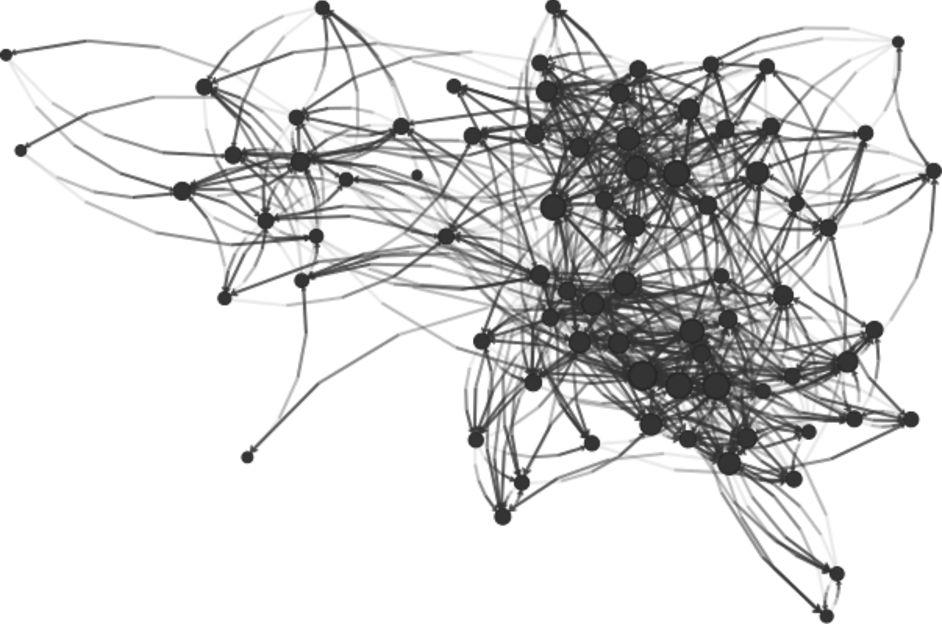
\includegraphics[width=1cm]{fig/ukfaculty.pdf} \name}
\pagestyle{fancy}
\fancyhead{}
\fancyfoot{}
\renewcommand{\headrulewidth}{0pt}
\fancyhead[L]{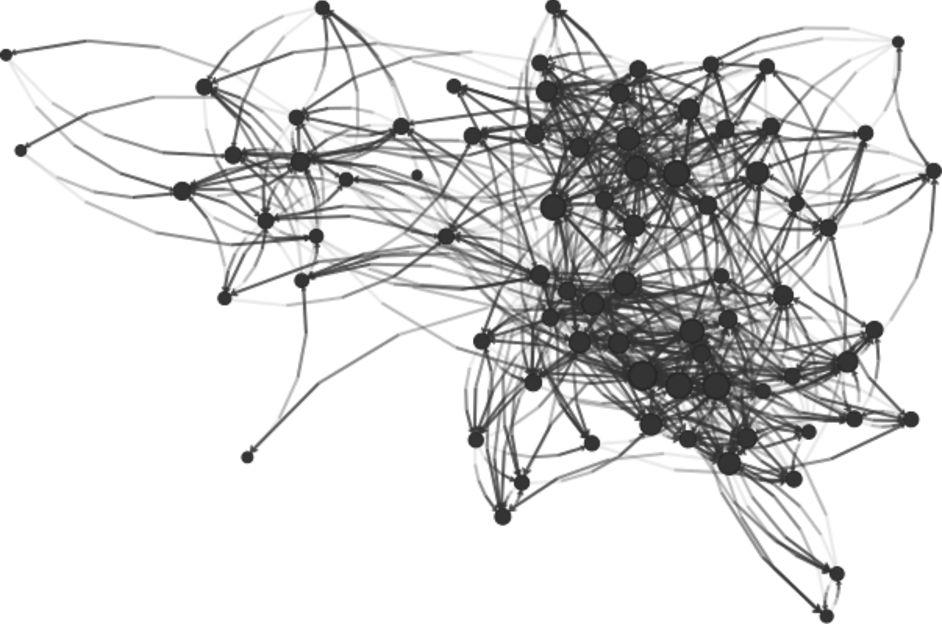
\includegraphics[width=1cm]{fig/ukfaculty.pdf}\\\vspace{-.75cm}\hspace{1.1cm}\emph{\name}}
\fancyhead[R]{\small\thepage}
\thispagestyle{empty}

% Custom section fonts
%\usepackage{sectsty}
%\sectionfont{\sffamily\mdseries\Large}
%\subsectionfont{\sffamily\mdseries\itshape\large}

% Other possible font commands include:
% rmfamily
% \ttfamily for teletype,
% \sffamily for sans serif,
% \bfseries for bold,
% \scshape for small caps,
% \normalsize, \large, \Large, \LARGE sizes.

% Don't indent paragraphs.
\setlength\parindent{0em}

% Make lists without bullets
%\renewenvironment{itemize}{
%  \begin{list}{}{
%    \setlength{\leftmargin}{0.45cm}
%  }
%}{
%  \end{list}
%}

% Para poder poner comandos genericos en tablas (en el inicio del argumento)
\usepackage{array}

\renewcommand{\bf}{\bfseries\color{teal}}
\renewcommand{\textbf}[1]{{\bfseries\color{teal}#1}}

\begin{document}

% Place name at left
% \hfill 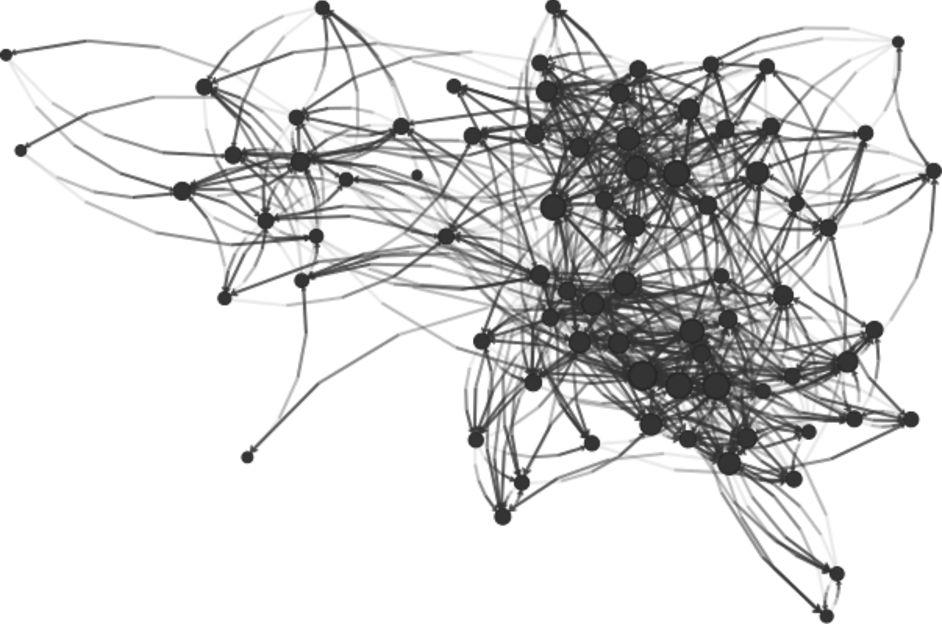
\includegraphics[width=.4\linewidth]{fig/ukfaculty.pdf}\vspace{-6cm}
\part*{\color{darkgray}{\name}}
% Alternatively, print name centered and bold:
%\centerline{\huge \bf \name}

%\vspace{0.25in}

\section*{Software Packages}

\begin{enumerate}[label={[}\arabic*{]},labelindent=5\parindent,labelsep=8pt]
\item \textbf{George G.} \textbf{Vega Yon}. \textit{defm: Estimation and simulation of Multi-binary response models} (2023). R package version 0.1.0. {\small URL}: \url{htps://cran.r-project.org/package=defm}. \\
\includegraphics[width=2.5cm]{fig/cran-downloads-defm.pdf} 
\item Derek Meyer, \textbf{George G.} \textbf{Vega Yon}. \textit{epiworldR: Fast Agent-Based Epi Models} (2023). R package version 0.0-2. {\small URL}: \url{https://cran.r-project.org/package=epiworldR}. \\
\includegraphics[width=2.5cm]{fig/cran-downloads-epiworldr.pdf} 
\item \textbf{George G.} \textbf{Vega Yon}. \textit{aphylo: Statistical Inference of Annotated Phylogenetic Trees} (2022). R package version 0.2-1. {\small URL}: \url{https://cran.r-project.org/package=aphylo}. \\
\includegraphics[width=2.5cm]{fig/cran-downloads-aphylo.pdf} 
\item \textbf{George G.} \textbf{Vega Yon}. \textit{A Flexible and General Agent Based Model Engine} (2022). C++ library version 0.0-1. {\small URL}: \url{https://github.com/UofUEpiBio/epiworld}.  
\item \textbf{George G.} \textbf{Vega Yon}. \textit{netplot: Beautiful graph drawing} (2021). R package version 0.1-1. {\small URL}: \url{https://cran.r-project.org/package=netplot}. \\
\includegraphics[width=2.5cm]{fig/cran-downloads-netplot.pdf} 
\item \textbf{George G.} \textbf{Vega Yon}. \textit{rgexf: Build, Import and Export GEXF Graph Files} (2020). R package version 0.16.0. {\small URL}: \url{https://CRAN.R-project.org/package=rgexf}. \\
\includegraphics[width=2.5cm]{fig/cran-downloads-rgexf.pdf} 
\item \textbf{George G.} \textbf{Vega Yon}, Thomas Valente. \textit{{{netdiffuseR: Analysis of Diffusion and Contagion Processes on Networks}}} (2020). R package version 1.22.0. {\small URL}: \url{https://github.com/USCCANA/netdiffuseR}. \\
\includegraphics[width=2.5cm]{fig/cran-downloads-netdiffuser.pdf} 
\item \textbf{George G.} \textbf{Vega Yon}, Kayla de la Haye. \textit{ergmito: Exponential Random Graph Models for Small Networks} (2020). R package version 0.3-0. {\small URL}: \url{https://cran.r-project.org/package=ergmito}. \\
\includegraphics[width=2.5cm]{fig/cran-downloads-ergmito.pdf} 
\item \textbf{George G.} \textbf{Vega Yon}. \textit{slurmR: A Lightweight Wrapper for 'Slurm'} (2020). R package version 0.4-1. {\small URL}: \url{https://CRAN.R-project.org/package=slurmR}. \\
\includegraphics[width=2.5cm]{fig/cran-downloads-slurmr.pdf} 
\item \textbf{George G.} \textbf{Vega Yon}. \textit{fmcmc: A friendly MCMC framework} (2020). R package version 0.3-0. {\small URL}: \url{https://CRAN.R-project.org/package=fmcmc}. \\
\includegraphics[width=2.5cm]{fig/cran-downloads-fmcmc.pdf} 
\item \textbf{George G.} \textbf{Vega Yon}. \textit{barry: your to-go motif accountant} (2020). C++ library version 0.0-1. {\small URL}: \url{https://github.com/USCbiostats/barry}.  
\item \textbf{George G.} \textbf{Vega Yon}. \textit{pruner: Implementing the Felsenstein's Tree Pruning algorithm} (2020). C++ library version 0.0-1. {\small URL}: \url{https://github.com/USCbiostats/pruner}.  
\item \textbf{George G.} \textbf{Vega Yon}, Brian Quistorff. \textit{parallel: Stata Module for Parallel Computing} (2019). Stata Module version 1.20.0. {\small URL}: \url{https://github.com/gvegayon/parallel}.  
\item \textbf{George G.} \textbf{Vega Yon}. \textit{googlePublicData: Working with Google's 'Public Data Explorer' DSPL Metadata Files} (2017). R package version 0.16.1. {\small URL}: \url{https://CRAN.R-project.org/package=googlePublicData}. \\
\includegraphics[width=2.5cm]{fig/cran-downloads-googlepublicdata.pdf} 
\item \textbf{George G.} \textbf{Vega Yon}, Enyelbert Mu~noz. \textit{ABCoptim: Implementation of Artificial Bee Colony (ABC) Optimization} (2017). R package version 0.15.0. {\small URL}: \url{https://CRAN.R-project.org/package=ABCoptim}. \\
\includegraphics[width=2.5cm]{fig/cran-downloads-abcoptim.pdf} 
\item \textbf{George G.} \textbf{Vega Yon}. \textit{{twitterreport: Out-of-the-box analysis and 
	reporting tools for twitter}} (2016). R package version 0.16. {\small URL}: \url{https://doi.org/10.5281/zenodo.44528}.  

\end{enumerate}



\section*{Peer Reviewed Publications}
\nocite{*}

\printbibliography[title=\vskip-20pt,keyword=published,resetnumbers=true]

\section*{Work in Progress and Technical Reports}

\printbibliography[title=\vskip-20pt,keyword=wip,resetnumbers=1]

\section*{Books}

\noindent ``Applied Network Science with R'' (on development) \url{https://book.ggv.cl/}

\noindent ``Applied HPC with R'' (on development) \url{https://book-hpc.ggv.cl/}



\bigskip

% Footer
\begin{center}
 \begin{footnotesize}
   last update: \today \\
   \href{\footerlink}{\texttt{\footerlink}}
 \end{footnotesize}
\end{center}

\end{document}

